\documentclass[12pt]{ctexart}
\usepackage{geometry}       % 设置页面整体布局
\geometry{top=2.5cm, bottom=2.5cm, left=2cm, right=2cm}
\usepackage{fancyhdr}       % 设置页眉页脚布局
\pagestyle{fancy}
\rhead{\thepage}            % 设置右页眉为页数
\chead{中国科学技术大学}
\cfoot{}                    % 设置中间页脚为空
\usepackage{amsmath}        % 数学公式宏包
\numberwithin{equation}{section}
\usepackage{esint}          % 交叉引用宏包
\usepackage[colorlinks,     % 设置引用的颜色
            linkcolor=black,
            anchorcolor=black,
            urlcolor=cyan,
            citecolor=black,
           ]{hyperref}
\usepackage{makecell}       % 插入表格宏包
\usepackage{longtable}      % 长表格宏包
\usepackage{appendix}       % 生成附录宏包
\usepackage{graphicx}       % 插入图片宏包
\usepackage{epstopdf}       % 插入eps图片宏包
\usepackage{cite}           % 文献引用宏包
\renewcommand{\thefigure}   % 设置图片编号格式
    {\thesection{}.\arabic{figure}}
\renewcommand{\thefootnote}{} % 设置角标编号不出现在文中
                            % 以\footnotetext{Footnotetext without footnote mark}使用
\usepackage{unicode-math}
\usepackage{listings}
\usepackage{hyperref}



\CTEXsetup[format={\Large\bfseries}]{section}

\begin{document}

\nocite{*}

\begin{center}
    \heiti \fontsize{24pt}{0}{电池电动势的测定和应用}

    \vspace{12pt}

    \kaishu \fontsize{13.75pt}{0}禤科材
    

    \footnotetext{\textbf{实验日期:}2022年9月23日}
    \footnotetext{\textbf{作者简介:}禤科材(2002-),男,学号PB20030874,中国科学技术大学本科在读,专业方向为化学物理}
    \footnotetext{\textbf{联系方式:}电话 18108064415 ,邮箱 \href{mailto:ustcxkc@mail.ustc.edu.cn}{ustcxkc@mail.ustc.edu.cn}}

    \vspace{5pt}

    \songti \fontsize{12pt}{0}(中国科学技术大学化学与材料科学学院,安徽 合肥 230026)
\end{center}

\noindent\textbf{摘~~~\!要}~~~\!
{化学反应电动势与许多热力学函数之间存在定量关系。由于电动势便于测量,
该优点使电动势的测量成为许多热力学函数的间接测量方法。本实验使用
对消法,将氧化还原反应做成电池反应,通过对原电池可逆电动势进行测量获得了一系列热力学参数。
实验还通过电动势的测量数据给出了难溶电解质的溶度积常数。此外还通过数理统计方法分析了电池极化对电动势的影响}
\newline
\textbf{关键字}~~~\!
{\kaishu 电动势;对消法;原电池;热力学函数}

\begin{center}
    {\Large\rmfamily\textbf{Measurement and Application of Battery Electromotive Force}}

    \vspace{12pt}

    {\slshape Xuan Kecai}

    \vspace{5pt}

    (School of Chemistry and Material Science, USTC, Hefei 230026, China)
\end{center}

\noindent\textbf{Abstract}~~~\!
{\linespread{0.5} There are quantitative corresponding relationships between chemical reaction electromotive forces and many thermodynamic
functions. For the convenience in measuring electromotive forces, this 
indirect measurement method is used for a wide range of thermodynamic functions.
In this experiment, the redox reaction was made into a battery reaction with the elimination method and a series of thermodynamic parameters were
obtained by measuring the reversible electromotive force of
the primary cell. The solubility product constant of insoluble
electrolyte was also calculated given the data of electromotive forces.In addition, the influence of battery polarization on electromotive force was tested by mathematical statistics methods.}
\newline
\textbf{Keywords}~~~\!
Electrodynamic force; Elimination method; Primary battery;
Thermodynamic function


\section{序言}
电池的电动势不能直接用伏特计来测量。因为把伏特计与电池接通后,
必须有适量的电流通过才能使伏特计显示。这样会使电极反应不可逆,
所测量结果为有“极化”现象发生时的外电压。要准确测量电池电动势只有
在电流无限小的可逆情况下进行,对消法可达到此目的$^{[1]}$。

使用电池电动势可以计算热力学量。对于一个氧化还原反应,利用电池反应
可以简单、准确的测量其焓变、熵变和Gibbs自由能变化。
\begin{align}
    \Delta_{\text{r}} G_{\text{m}}^{\ominus} &= -nFE, \\
    \Delta_{\text{r}} S_{\text{m}}^{\ominus}
        &= nF\left(\frac{\partial E}{\partial T}\right)_p, \\
    \Delta_{\text{r}} H_{\text{m}}^{\ominus}
        &= \Delta_{\text{r}} G_{\text{m}}^{\ominus}
        + T \Delta_{\text{r}} S_{\text{m}}^{\ominus}.
\end{align}

此外,根据下式还可以计算难溶物的溶度积常数。
\begin{align}
    E = \frac{RT}{F}
    \ln\frac{a_{\mathrm{Ag^+}}a_{\mathrm{Cl^-}}}
        {K_{\text{sp}}}.
\end{align}

\section{实验}
\subsection{试剂与仪器}
琼脂粉(BR,国药集团化学试剂有限公司),KNO$_3$(AR,国药集团化学试剂
有限公司),KCl溶液(0.1 mol/L),银电镀液(0.1 mol/L的AgNO$_3$溶液,
CuCl$_2$溶液(0.1 mol/L),铜电镀液(0.1 mol/L的CuSO$_4$ 溶液)。

HK-2A型超级恒温水浴(南京南大万和科技有限公司)、EM-3D 型数字式
电子电位差计、Ag-AgCl 参比电极,铂电极,铜电极,银电极,标准电池,
半电池管,毫安表,电阻箱,U 型管,直流稳压电源,检流计,导线等。

\subsection{实验方法}
(1)接好线路,调节可变电阻,将银电极在9 V下镀银20 min,并迅速放入
0.1000 M AgNO$_3$溶液的半电池管中,将铜电极在15 V 在镀铜60 min,并
迅速放入0.1000 M CuSO$_4$溶液的半电池管电极。

(2)取3 g琼脂粉和120 mL饱和硝酸钾溶液放于锥形瓶中,水浴加热使其
变成粘稠状液体,预热后用吸量管向U 型管加入粘稠状液体,自然冷却凝固。
使管口呈凸面。

(3)组装电池,校准电位差计。将上述制备的银电极与制备好的铜电极组成
电池,将恒温槽置于30$^\circ$C 恒温15min 后测量该电池的电动势三次。

(4)将上述制备的银电极与Ag-AgCl 参比电极组成电池,分别在
30$^\circ$C、35$^\circ$C、40$^\circ$C 和45$^\circ$C下测量
该电池的电动势。

\section{结果与讨论}
\subsection{实验结果}
\subsubsection{Cu-Ag 原电池计算结果}
电池表达式为
\begin{align}
    \mathrm{Cu(s)}|\mathrm{CuCl_2}(0.1000 \mathrm{M})
    ||\mathrm{AgNO_3}(0.1000 \mathrm{M})|\mathrm{Ag(s)}.
\end{align}

在303.15 K下测得该电池的电动势为438.554 mV,理论计算值$^{[2]}$
为441.958 mV,相对误差为-0.77\%。误差较小,结果可靠。

各组实验数据相对均值的偏差用 Mathematica 绘图如下:
\begin{figure}[ht]
    \centering
    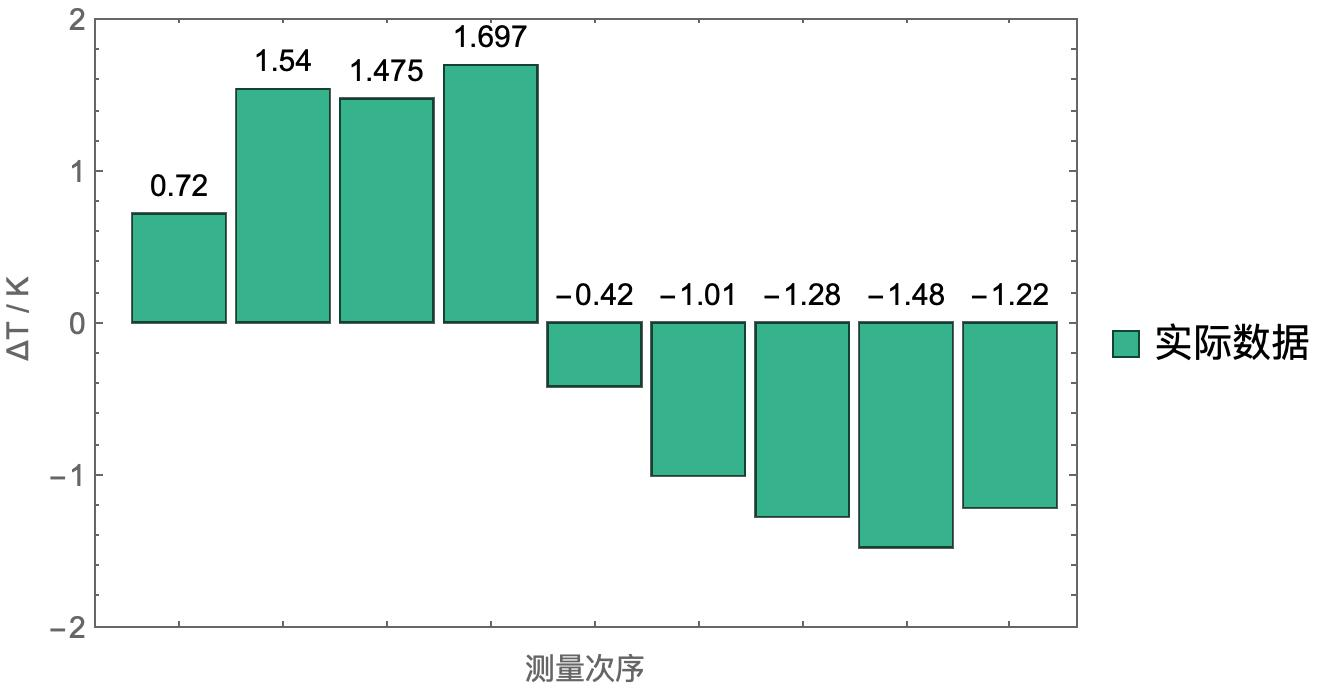
\includegraphics[width=0.9\textwidth]{Figure_3.jpg}
    \caption{实验数据相对均值的偏差}
    \label{fig:bar}
\end{figure}

实验数据密度直方图与对应正态概率密度函数如图 \ref*{fig:histo} 所示,直观看来所得实验数据并不服从正态分布,应当存在某种确定性的因素影响着实验结果。设原假设 $H_0:$ 实验数据服从一定的 正态分布,对原始数据做 Kolmogorov-Smirnov 拟合优度检验,P-Value 为 0.21229,实际分布服从正态分布的概率很小,放弃原假设。

经分析,原电池容易极化,极化程度随电池使用时间的增加而增加,而电池电动势随极化程度的增加而下降。根据实验所得,可以合理推测数据与正态分布的偏差是由电池的极化效应导致的。


\begin{figure}[ht]
    \centering
    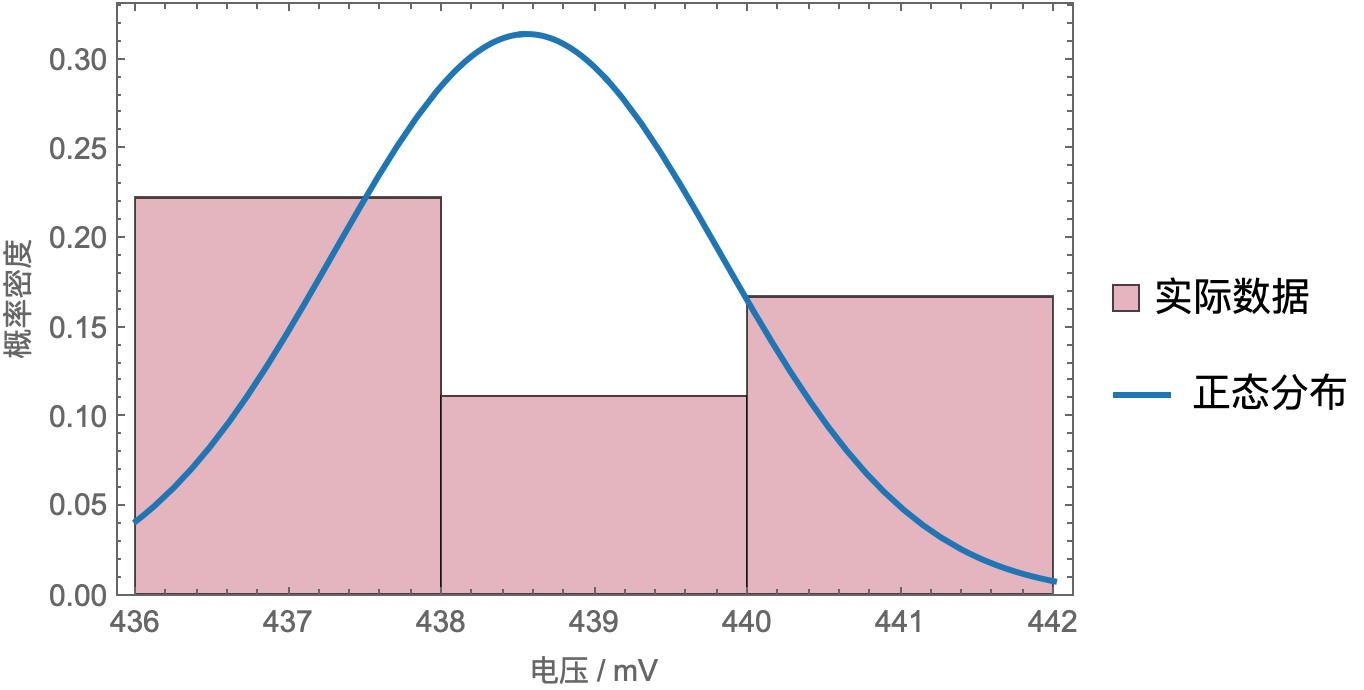
\includegraphics[width=0.8\textwidth]{Figure_2.jpg}
    \caption{数据直方图与正态密度对比}
    \label{fig:histo}
\end{figure}

\subsubsection{Ag-AgCl 原电池计算结果}
电池表达式为
\begin{align}
    \mathrm{Ag-AgCl(s)}|\mathrm{KCl}(0.1000 \mathrm{M})
    ||\mathrm{AgNO_3}(0.1000 \mathrm{M})|\mathrm{Ag(s)}.
\end{align}

在不同温度下测定电池电动势并做$E \sim T$图,用 Mathematica 对曲线进行
线性拟合得到拟合函数如下

\begin{align}
E = 690.082 - 0.8182 T 
\end{align}

拟合图像如图 \ref*{fig:linear} 所示。

\begin{figure}[!h]
    \centering
    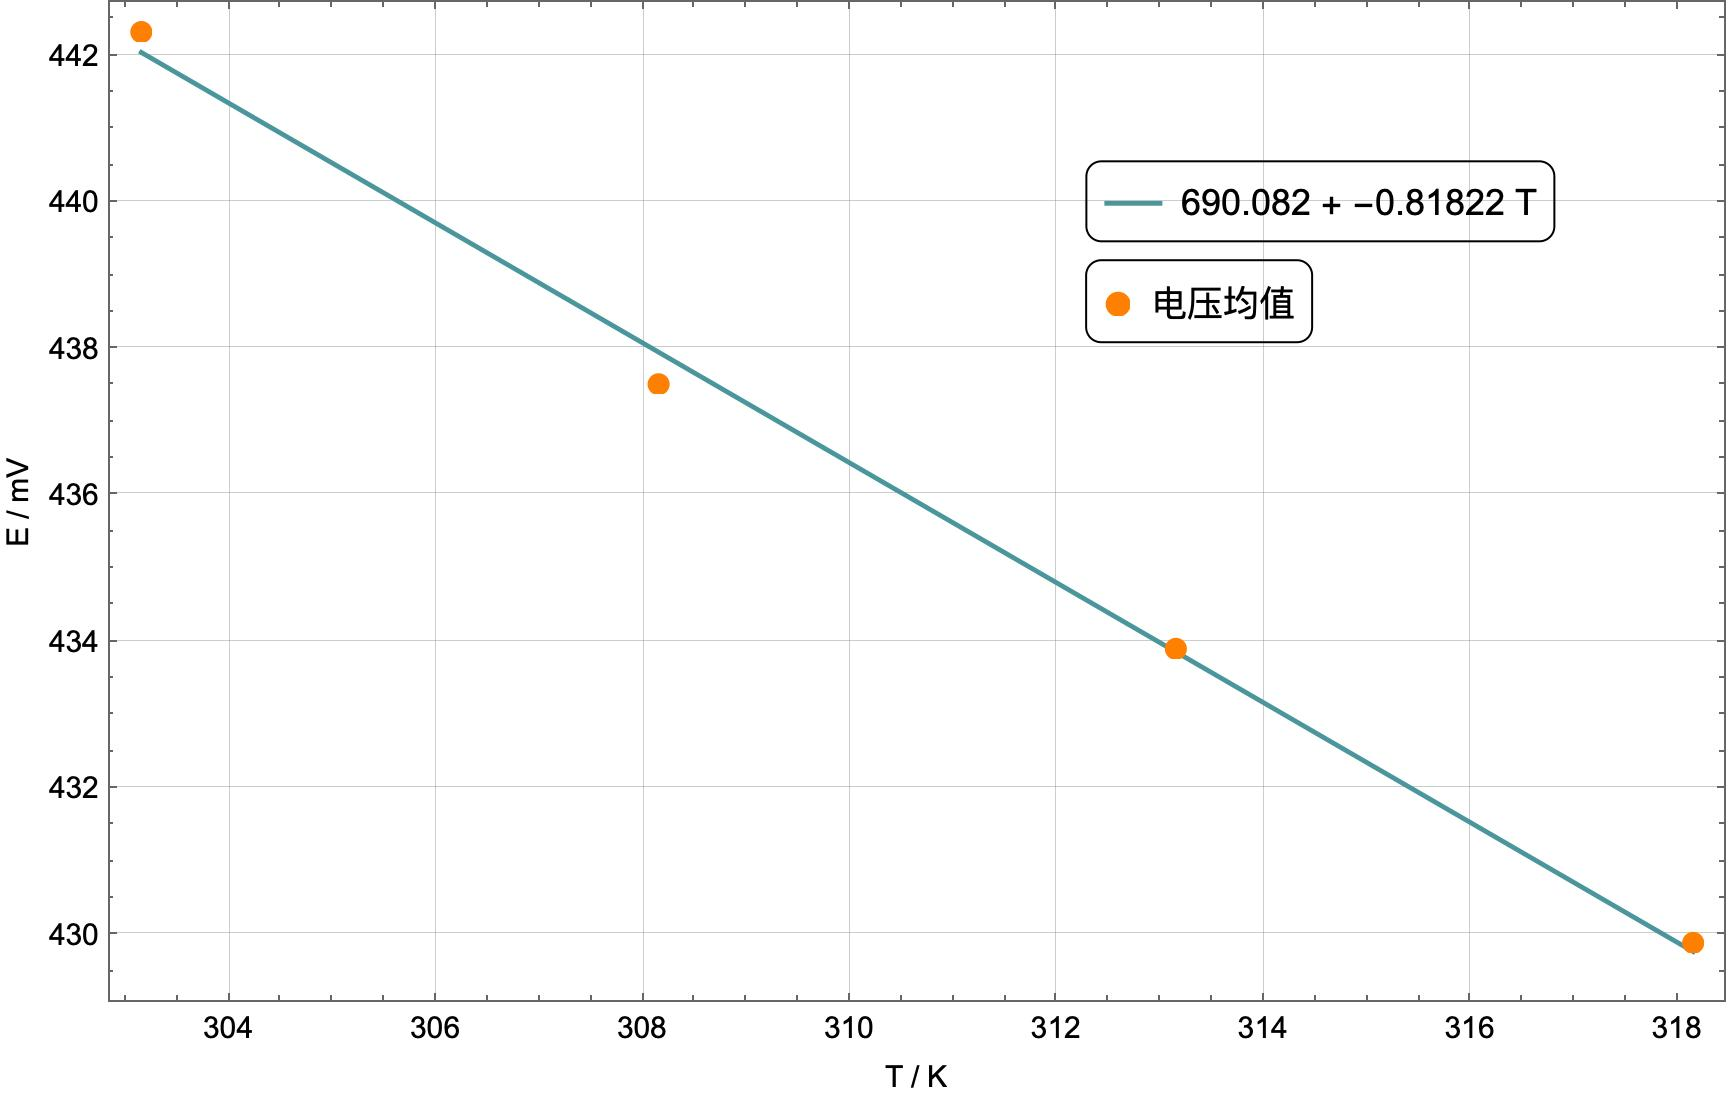
\includegraphics[scale=0.4]{Figure_1.jpg}
    \caption{Ag-AgCl 原电池的 E-T 拟合曲线}
    \label{fig:linear}
\end{figure}

故该电池的温度系数$\partial E/\partial T$为 -0.8182 mV/K,
该反应的标准熵变$\Delta_r S^{\ominus}_{\text{m}}$为 -78.94 J/
(mol$\cdot$K),标准电动势$E^{\ominus}$为 446.154 mV,标准 Gibbs
自由能变$\Delta_r G^{\ominus}_{\text{m}}$为 -43.04 kJ/mol,标准
焓变$\Delta_r H^{\ominus}_{\text{m}}$为 -66.58 kJ/mol。用相同的
方法可以计算出四个温度下的$\Delta_r H_{\text{m}}$、
$\Delta_r G_{\text{m}}$和$\Delta_r S_{\text{m}}$如表 1 所示。

\begin{longtable}{ccccc}
    \caption{不同温度下的$\Delta_r H_\text{m}$、$\Delta_r G_\text{m}$与$\Delta_r S_\text{m}$} \\
    \hline
    温度/K & 电动势/mV & $\Delta_r G_\text{m}$ / $\mathrm{(kJ\cdot mol^{-1})}$ & $\Delta_r H_\text{m}$ / $\mathrm{(kJ\cdot mol^{-1})}$ & $\Delta_r S_\text{m}$ / $\mathrm{(kJ\cdot mol^{-1}\cdot K^{-1})}$ \\
    \hline
    303.15 & 442.039 & -42.65 & -66.58 & -78.94 \\
    308.15 & 437.948 & -42.25 & -66.58 & -78.94 \\
    313.15 & 433.857 & -41.86 & -66.58 & -78.94 \\
    318.15 & 429.766 & -41.46 & -66.58 & -78.94 \\
    \hline
\end{longtable}

\newpage
经过理论计算得到30.00$^\circ$C下的三个热力学量分别为$\Delta G$ =
-42.34 kJ/mol、$\Delta H$ = -64.57 kJ/mol、$\Delta S$ =
-73.18 J/(mol$\cdot$K),相对误差分别为0.7\%、
3.1\% 和7.8\%。

\subsubsection{\texorpdfstring{AgCl 溶度积常数$K_{\text{sp}}$的计算}{}}

经实验数据计算得 $K_{\text{sp}}$ = 2.53$\times$10$^{-10}$,
$pK_{\text{sp}}$ = 9.60,查表得标准数据为$K_{\text{sp}}$ =
1.8$\times$10$^{-10}$,$pK_{\text{sp}}$ = 9.74,$K_{\text{sp}}$
和$pK_{\text{sp}}$的相对误差分别为9.8\%
和0.41\%。

\subsection{误差分析}
\subsubsection{系统误差}
(1)单一阴阳离子的活度无法测得,采用平均活度代替,会引入一定的误差。

(2)恒温槽温度读数精度和温度的波动会引起一定的误差。

(3)计算时假定各热力学量在一定温度范围内不随温度变化,带来一定的误差。

(4)实验过程中大气压强并不是精确的恒定值。

(5)电极的极化随电路通电时间的延长而增强,导致实验中平行测量的
数据呈递减趋势。

(6)电极在空气中会有不可避免的氧化现象,会引起一定的实验误差。

\subsubsection{偶然误差}
(1)测量时,两条导线的接触情况可能使接触处的电阻有略微不同,导致
测得的电动势有微小的差别。

(2)制备琼脂时缺乏搅拌,仅用摇晃容器代替,可能会导致溶质扩散不均匀。
造成对盐桥中离子迁移速率的影响。

(3)电解液和半电池液的浓度难以做到精确的0.1000 mol/L。

\subsection{实验改进与思考}

打磨银棒时要在不磨损掉太多银的情况下尽可能打磨干净,否则会导致电镀
效果较差,使得后面测电压时电压不稳定。使用电位差计时在非测量状态下
要断开电路,防止过多的电荷通过标准电池或被测电池,造成极化现象的
加重,破坏被测电池的可逆性,影响测量数据的准确性。

\subsection{不可逆电池的电动势}

事实上“可逆电池”只是最理想的情况,认为电池反应以可逆的形式发生。但现实中并不存在完全可逆的电池,原则上只能调控反应条件,使得电池反应缓慢地进行,此时的电池则处于“准静态”,是最接近“可逆”的状态,而本实验使用的对消法即是这样的设计。

所以对于不可逆电池,我们总是可以通过控制反应发生的速率来使得反应更加接近一个可逆反应,比如在低温、低压等可以减缓电池的反应的条件下测定电池的电动势,。



\section{结语}
本实验使用对消法测量了不同温度下的电池电动势,并计算了氧化还原反应的
热力学量以及 AgCl 的溶度积常数。经计算在 303.15 K 下 Cu-Ag 电池的
电动势为 438.554 mV,理论计算值为 441.958 mV,相对误差为 -0.77\%。
对实验数据进行 Kolmogorov-Smirnov 拟合优度检验,不可认为原始数据服从正态分布,
统计上可以认为存在确定性的因素对实验进行干扰。分析表明这种干扰来自电池的极化。

Ag-AgCl 电池反应的三个热力学量分别为 $\Delta G$ = -42.65 kJ/mol、
$\Delta H$ = -66.58 kJ/mol、$\Delta S$ = -78.94 J/(mol$\cdot$K),
与理论值$\Delta G$ = -42.34 kJ/mol、$\Delta H$ = -64.57 kJ/mol、
$\Delta S$ = -73.18 J/(mol$\cdot$K),相对误差分别为0.7\%、
3.1\% 和7.8\%。

经实验数据计算得到 AgCl 的$K_{\text{sp}}$ =
1.624$\times$10$^{-10}$,$pK_{\text{sp}}$ = 9.79,查表得标准数据
为$K_{\text{sp}}$ = 1.8$\times$10$^{-10}$,$pK_{\text{sp}}$ =
9.74,$K_{\text{sp}}$和$pK_{\text{sp}}$的相对误差分别为9.8\%
和0.41\%。数据误差较小,结果可靠。


\begin{center}
    \Large\bfseries{参考文献}
\end{center}
\noindent
[1] 傅献彩, 沈文霞, 姚天扬等. 物理化学(第五版). 上册[M].
高等教育出版社,2006.

\noindent
[2] J.A. 迪安, 迪安, Dean, et al. 兰氏化学手册 [M]. 科学出版社,
2003.

\newpage

\begin{center}
    \LARGE\bfseries{附录~~~实验数据处理}
\end{center}
\begin{center}
    \Large\bfseries{附录I~~~实验数据处理}
\end{center}

\subsection*{I.1~~~Cu-Ag 原电池的计算}

电池表达式为
\begin{align}
    \mathrm{Cu(s)}|\mathrm{CuCl_2}(0.1000 \mathrm{M})
    ||\mathrm{AgNO_3}(0.1000 \mathrm{M})|\mathrm{Ag(s)}.
    \tag{I.1}
\end{align}

电池总反应,正负极反应分别为
\begin{align}
    \mathrm{2 Ag^{+} + Cu }&\mathrm{\longrightarrow Cu^{2+} + 2Ag}
    \tag{I.2} \\
    \mathrm{2 Ag^{+} + 2 e^{-} }&\mathrm{\longrightarrow 2 Ag}
    \tag{I.3} \\
    \mathrm{Cu }&\mathrm{\longrightarrow Cu^{2+} + 2 e^{-}}
    \tag{I.4}
\end{align}

在0.1 M 的溶液里,近似认为$m = c$. 假定同一溶液中阴阳离子活度系数
相等。则
\begin{align}
    \gamma_{\mathrm{Ag^+}} = \gamma_{\mathrm{AgNO_3}} = 0.734
    \qquad
    \gamma_{\mathrm{Cu^+}} = \gamma_{\mathrm{CuCl_2}} = 0.154.
    \tag{I.5}
\end{align}

故电动势的理论值为
\begin{align}
    E(298.15 \mathrm{K}) &= E^{\ominus} + \frac{RT}{nF}
    \ln\frac{a_{\mathrm{Ag^+}^2}}{a_{\mathrm{Cu^{2+}}}}
    \notag \\
    &= E^\ominus + \frac{RT}{nF}\ln
    \frac{\gamma_{\mathrm{Ag^+}}^2 \cdot m_{\mathrm{Ag^+}}^2}
    {\gamma_{\mathrm{Cu^+}} \cdot m_{\mathrm{Cu^{2+}}}}
    \tag{I.6} \\
    &= 446.511 ~\mathrm{mV}. \notag
\end{align}

实验在303.15 K下进行,该温度下电池的电动势为
\begin{align}
    E(303.15 \mathrm{K}) = E(298.15 \mathrm{k})
    + \frac{\Delta T \Delta_r S^{\ominus}_\text{m}}{nF}
    = 441.958~\mathrm{mV}. \tag{I.7}
\end{align}

实验测量电动势的平均值为438.554 mV,故相对误差为-0.77\%。
实验误差较小,结果较为可靠。

各组数据密度直方图与对应正态概率密度函数如图 \ref*{fig:histo*} 所示,直观看来所得实验数据并不服从正态分布,应当存在某种确定性的因素影响着实验结果。设原假设 $H_0:$ 实验数据服从一定的正态分布,为对原始数据做 Kolmogorov-Smirnov 拟合优度检验,将下列代码输入Mathematica:

\begin{lstlisting}
    exp={439.278, 440.094, 440.029, 440.251, 
        438.129, 437.54, 437.268, 437.069, 437.33};
    H = DistributionFitTest[exp, Automatic, "HypothesisTestData"];
    H["TestDataTable"]
\end{lstlisting}

输出表格如下:

\begin{longtable}{|c|c|c|}
    \hline
     & Statistic & P-Value \\
    \hline
     Kolmogorov-Smirnov & 0.232174 & 0.21229\\
    \hline
\end{longtable}

P-Value 为 0.21229,实际分布服从正态分布的概率很小,放弃原假设。

经分析,原电池容易极化,极化程度随电池使用时间的增加而增加,而电池电动势随极化程度的增加而下降。根据实验所得,可以合理推测数据与正态分布的偏差是由电池的极化效应导致的。

\begin{figure}[ht]
    \centering
    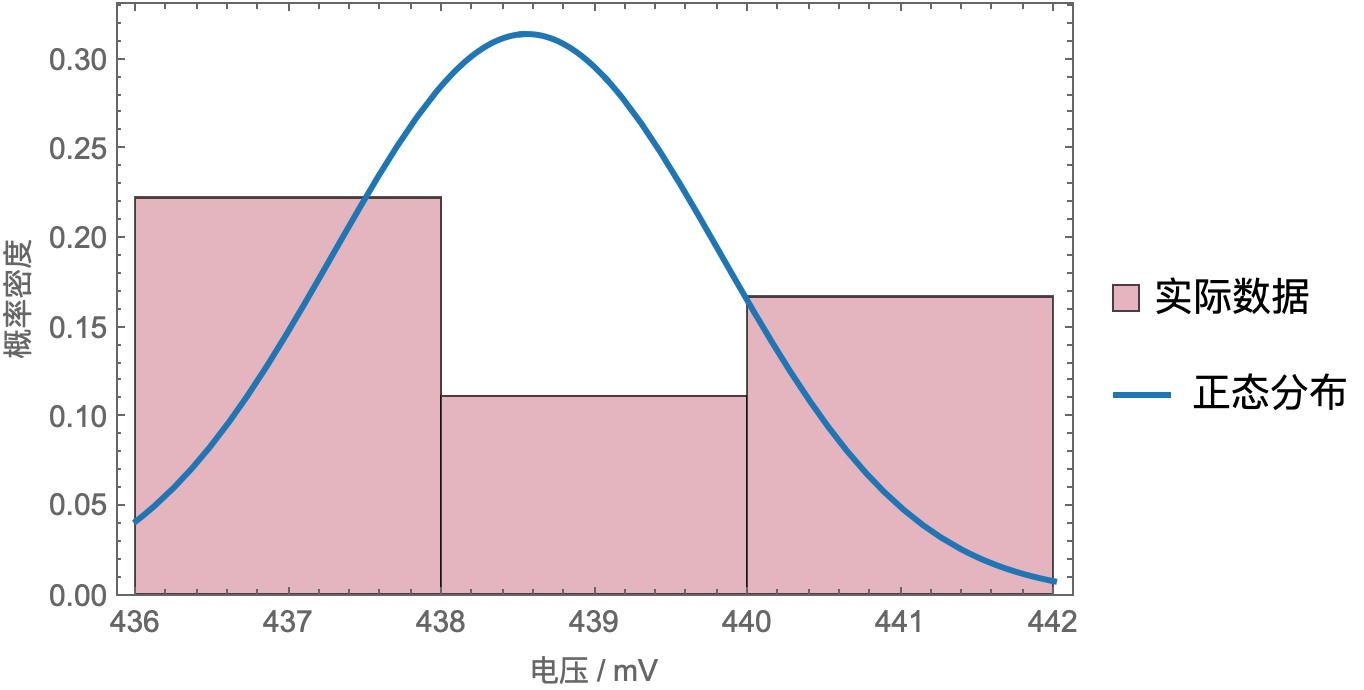
\includegraphics[width=0.7\textwidth]{Figure_2.jpg}
    \caption{数据直方图与正态密度对比}
    \label{fig:histo*}
\end{figure}


\subsection*{I.2~~~Ag-AgCl 原电池的计算}

电池表达式为

\begin{align}
    \mathrm{Ag-AgCl(s)}|\mathrm{KCl}(0.1000 \mathrm{M})
    ||\mathrm{AgNO_3}(0.1000 \mathrm{M})|\mathrm{Ag(s)}.
    \tag{I.8}
\end{align}

电池总反应,正负极反应分别为
\begin{align}
    \mathrm{Ag^{+} + Cl^{-} }&\mathrm{\longrightarrow AgCl}
    \tag{I.9} \\
    \mathrm{Ag^{+} + e^{-} }&\mathrm{\longrightarrow Ag}
    \tag{I.10} \\
    \mathrm{Ag + Cl^{-} }&\mathrm{\longrightarrow AgCl + e^{-}}
    \tag{I.11}
\end{align}

在不同温度下测定电池的电动势,并用 E 对 T 作图,用 Mathematica 进行
线性拟合,得到图像如图 \ref*{fig:fit} 所示。

\begin{figure}[htbp]
    \centering
    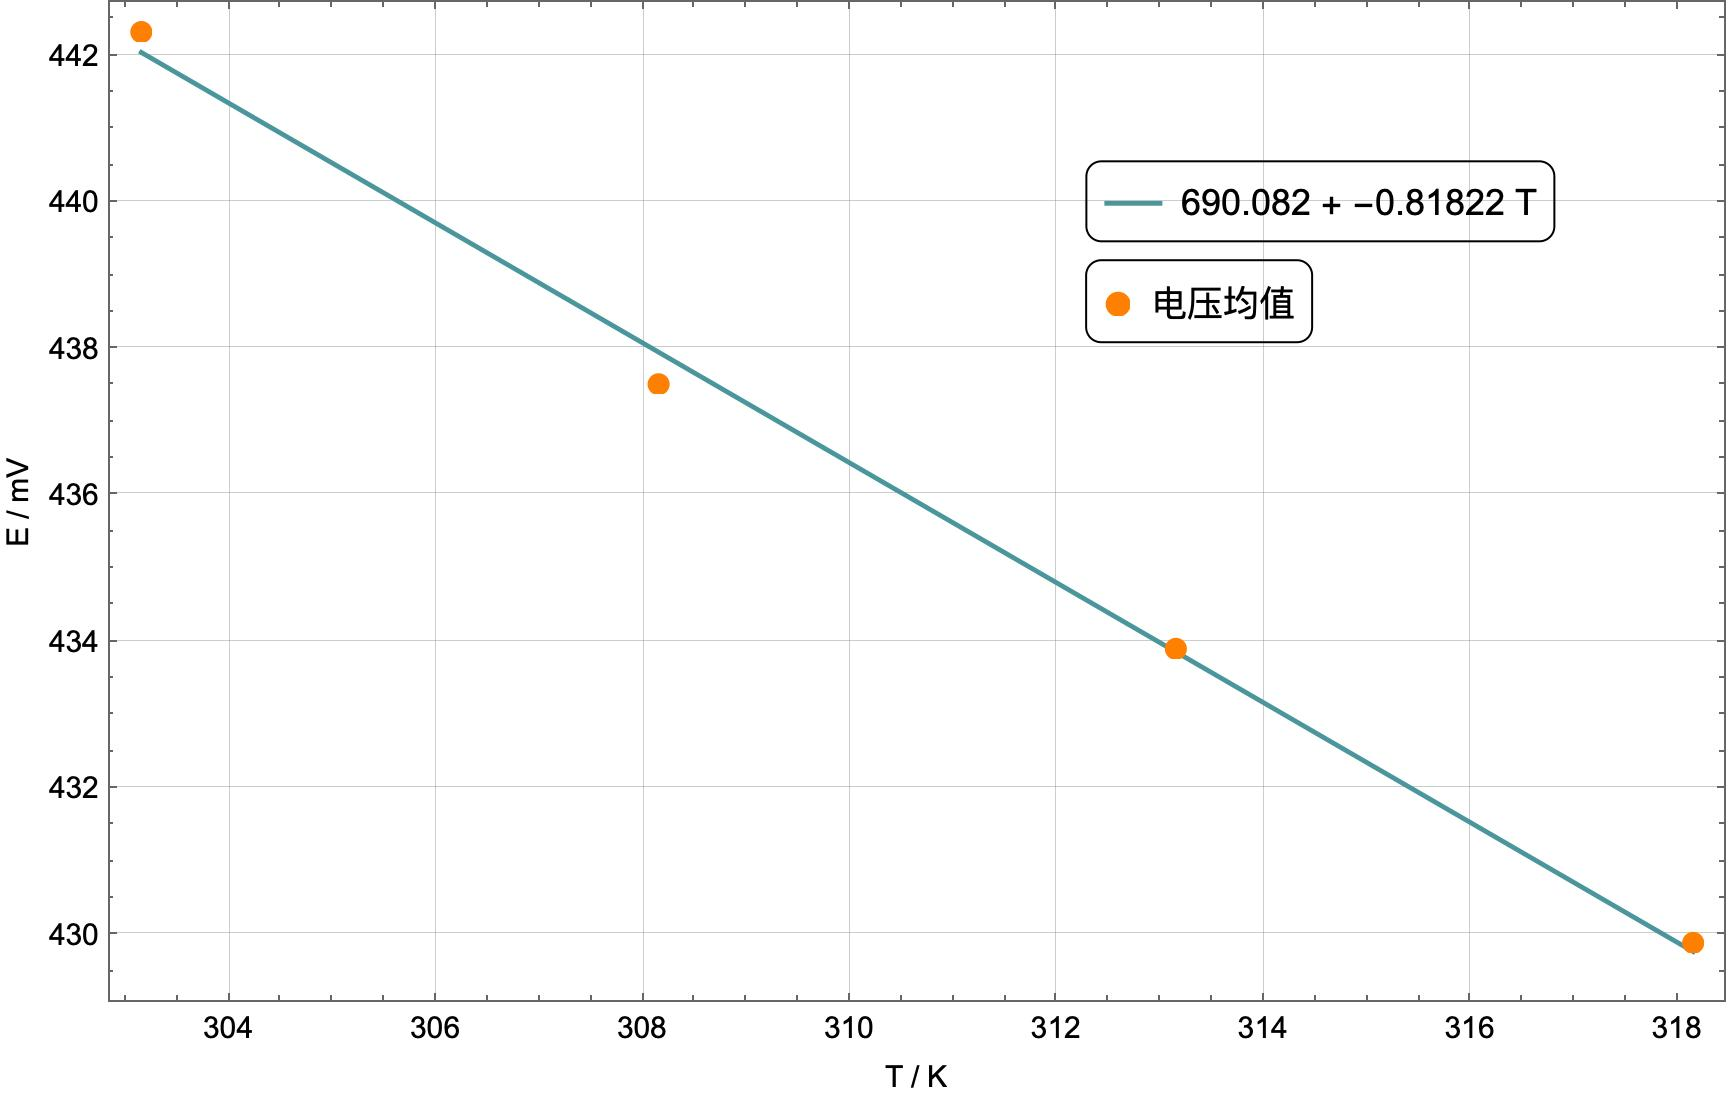
\includegraphics[scale=0.4]{Figure_1.jpg}
    \caption{Ag-AgCl 原电池的 E-T 拟合曲线}
    \label{fig:fit}
\end{figure}

拟合函数为
\begin{align}
    E = 690.082- 0.8182 T  \tag{I.12}
\end{align}

由斜率可得温度系数为
\begin{align}
    \left(\frac{\partial E}{\partial T}\right)_p
    = - 0.8182~\mathrm{mV/K}. \tag{I.13}
\end{align}

故该反应的熵变为
\begin{align}
    \Delta_r S_\text{m}^\ominus = nF
    \left(\frac{\partial E}{\partial T}\right)_p
    =-78.94~\mathrm{J\cdot mol^{-1}\cdot K^{-1}}. \tag{I.14}
\end{align}

将$T = 298.15$ K 带入拟合的函数得到反应电动势为
\begin{align}
    E^\ominus = -0.8182 \times 298.15 + 690.082 = 446.154
    ~\mathrm{(mV)}. \tag{I.15}
\end{align}

故反应的标准吉布斯自由能变为
\begin{align}
    \Delta_r G_\text{m}^\ominus = -nFE^\ominus = -43.04
    ~\mathrm{kJ/mol}. \tag{I.16}
\end{align}

反应的焓变为
\begin{align}
    \Delta_r H_\text{m}^\ominus = \Delta_r G_\text{m}^\ominus
        + T \Delta_r S_\text{m}^\ominus = -66.58
    ~\mathrm{kJ/mol}. \tag{I.17}
\end{align}

同理,可以算出其他温度下的$\Delta_r H_\text{m}$、
$\Delta_r G_\text{m}$、$\Delta_r S_\text{m}$的值,如表1所示。

\begin{longtable}{ccccc}
    \caption{不同温度下的$\Delta_r H_\text{m}$、$\Delta_r G_\text{m}$与$\Delta_r S_\text{m}$} \\
    \hline
    温度/K & 电动势/mV & $\Delta_r G_\text{m}$ / $\mathrm{(kJ\cdot mol^{-1})}$ & $\Delta_r H_\text{m}$ / $\mathrm{(kJ\cdot mol^{-1})}$ & $\Delta_r S_\text{m}$ / $\mathrm{(kJ\cdot mol^{-1}\cdot K^{-1})}$ \\
    \hline
    303.15 & 442.039 & -42.65 & -66.58 & -78.94 \\
    308.15 & 437.948 & -42.25 & -66.58 & -78.94 \\
    313.15 & 433.857 & -41.86 & -66.58 & -78.94 \\
    318.15 & 429.766 & -41.46 & -66.58 & -78.94 \\
    \hline
\end{longtable}

根据公式可以将298.15 K 下的标准数据换算为其他温度下的热力学数据。
下表为不同物质在298.15 K 下的标准热力学数据。

\begin{table}[!h]
\begin{center}
\caption{不同物质的标准$\Delta_r H_\text{m}$、$\Delta_r G_\text{m}$、$\Delta_r S_\text{m}$}
\begin{tabular}{ p{1cm}<{\centering} p{1cm}<{\centering} p{3cm}<{\centering} p{3cm}<{\centering} p{3.5cm}<{\centering} p{3.5cm}<{\centering} }
    \hline
    物质 & 状态 & $\Delta_r G_\text{m}$ / $\mathrm{(kJ\cdot mol^{-1})}$ & $\Delta_r H_\text{m}$ / $\mathrm{(kJ\cdot mol^{-1})}$ & $\Delta_r S_\text{m}$ / $\mathrm{(kJ\cdot mol^{-1}\cdot K^{-1})}$ & $C_{p, m}$ / $\mathrm{(kJ\cdot mol^{-1}\cdot K^{-1})}$ \\
    \hline
    AgCl   & s  & -109.8 & -127.0 & 96.3 &   50.8 \\
    Ag$^+$ & aq &   77.1 &  105.6 & 72.7 &   21.8 \\
    Cl$^-$ & aq & -131.2 & -167.2 & 56.7 & -136.4 \\
    \hline
\end{tabular}
\end{center}
\end{table}

由此可以计算得出
\begin{align}
    \Delta_r G_\text{m}^\ominus &= -55.7~\mathrm{kJ/mol},
    \tag{I.18} \\
    \Delta_r H_\text{m}^\ominus &= -65.4~\mathrm{kJ/mol},
    \tag{I.19} \\
    \Delta_r S_\text{m}^\ominus &= -32.9
    ~\mathrm{J\cdot mol^{-1}\cdot K^{-1}}, \tag{I.20} \\
    C_{p, m}^\ominus &= 165.4
    ~\mathrm{J \cdot mol^{-1} \cdot K^{-1}}. \tag{I.21}
\end{align}

对于其他温度的热力学函数值,采用如下公式计算
\begin{align}
    \Delta_r S_\text{m}(T) &= \Delta_r S_\text{m}(298.15
    ~\mathrm{K}) + \int_{298.15~\mathrm{K}}^{T}
    \frac{C_{p, m}}{T}\mathrm{d}T, \tag{I.22} \\
    \Delta_r H_\text{m}(T) &= \Delta_r H_\text{m}(298.15
    ~\mathrm{K}) + \int_{298.15~\mathrm{K}}^{T}C_{p, m}
    \mathrm{d}T, \tag{I.23} \\
    \Delta_r G_\text{m}(T) &= \Delta_r H_\text{m}(T)
    - T\Delta_r S_\text{m}(T). \tag{I.24}
\end{align}

再考虑活度的修正,有
\begin{align}
    \Delta_r S(T) &= \Delta_r S_\text{m}(T)
    + R\ln(a_{\mathrm{Ag^+}}a_{\mathrm{Cl^-}}), \tag{I.25} \\
    \Delta_r G(T) &= \Delta_r G_\text{m}(T)
    - R\ln(a_{\mathrm{Ag^+}}a_{\mathrm{Cl^-}}), \tag{I.26} \\
    \Delta_r H(T) &= \Delta_r G_\text{m}(T)
    + T \Delta_r S_\text{m}(T). \tag{I.27}
\end{align}
其中$\gamma_{\mathrm{Ag^+}} = 0.734$,$\gamma_{\mathrm{Cl^-}} = 0.770$。

计算结果如表 4 所示。

\begin{longtable}{|c|c|}
    \caption{计算结果} \\
    \hline
    $\Delta_r H_\text{m}(303.15K)$ & -64.57 kJ/mol \\
    \hline
    $\Delta_r S_\text{m}(303.15K)$ & -30.15 J$\cdot$mol$^{-1}\cdot$K$^{-1}$ \\
    \hline
    $\Delta_r G_\text{m}(303.15K)$ & -55.43 kJ/mol \\
    \hline
    $\Delta_r H(303.15K)$ & -64.57 kJ/mol \\
    \hline
    $\Delta_r S(303.15K)$ & -73.18 J$\cdot$mol$^{-1}\cdot$K$^{-1}$ \\
    \hline
    $\Delta_r G(303.15K)$ & -42.34 kJ/mol \\
    \hline
\end{longtable}

由此可得,实验所得$\Delta G$、$\Delta H$、$\Delta S$的相对误差
分别为0.7\%、3.1\%、7.8\%。

\subsection*{I.2~~~AgCl 溶度积常数的计算}

电动势和溶度积常数之间的关系式为
\begin{align}
    E = \frac{RT}{F}\ln
    \frac{a_{\mathrm{Ag^+}}a_{\mathrm{Cl^-}}}{K_{sp}}.
    \tag{I.28}
\end{align}

由此可得
\begin{align}
    K_{\mathrm{sp}} = 1.62407\times 10^{-10},
    \tag{I.29} \\
    pK_{\mathrm{sp}} = 9.79. \tag{I.30}
\end{align}

查表得标准数据为$K_{\mathrm{sp}} = 1.8\times 10^{-10}$,
$pK_{\mathrm{sp}} = 9.74$。故相对误差分别为9.8\%,0.41\%。

\pagebreak

\begin{center}
    \Large\bfseries{附录II~~~原始数据记录}
\end{center}

\begin{longtable}{|c|c|c|c|c|c|c|c|c|c|}
    \caption{Cu-Ag电动势测定} \\
    \hline
    测量序号 & 1 & 2 & 3 & 4 & 5 \\
    \hline
    电动势$E_1$/mV & 439.278& 440.094& 440.029& 440.251& 438.129\\
    \hline
    测量序号 & 6 & 7 & 8 & 9 &  \\
    \hline
    电动势$E_1$/mV & 437.540& 437.268& 437.069& 437.330 & \\
    \hline
    电动势平均值$\overline{E}_1$/mV & \multicolumn{5}{c|}{438.554} \\
    \hline
    电动势理论值$E_T$/mV & \multicolumn{5}{c|}{441.958} \\
    \hline
    相对误差 & \multicolumn{5}{c|}{-0.77\%} \\
    \hline
\end{longtable}

\begin{figure}[ht]
    \centering
    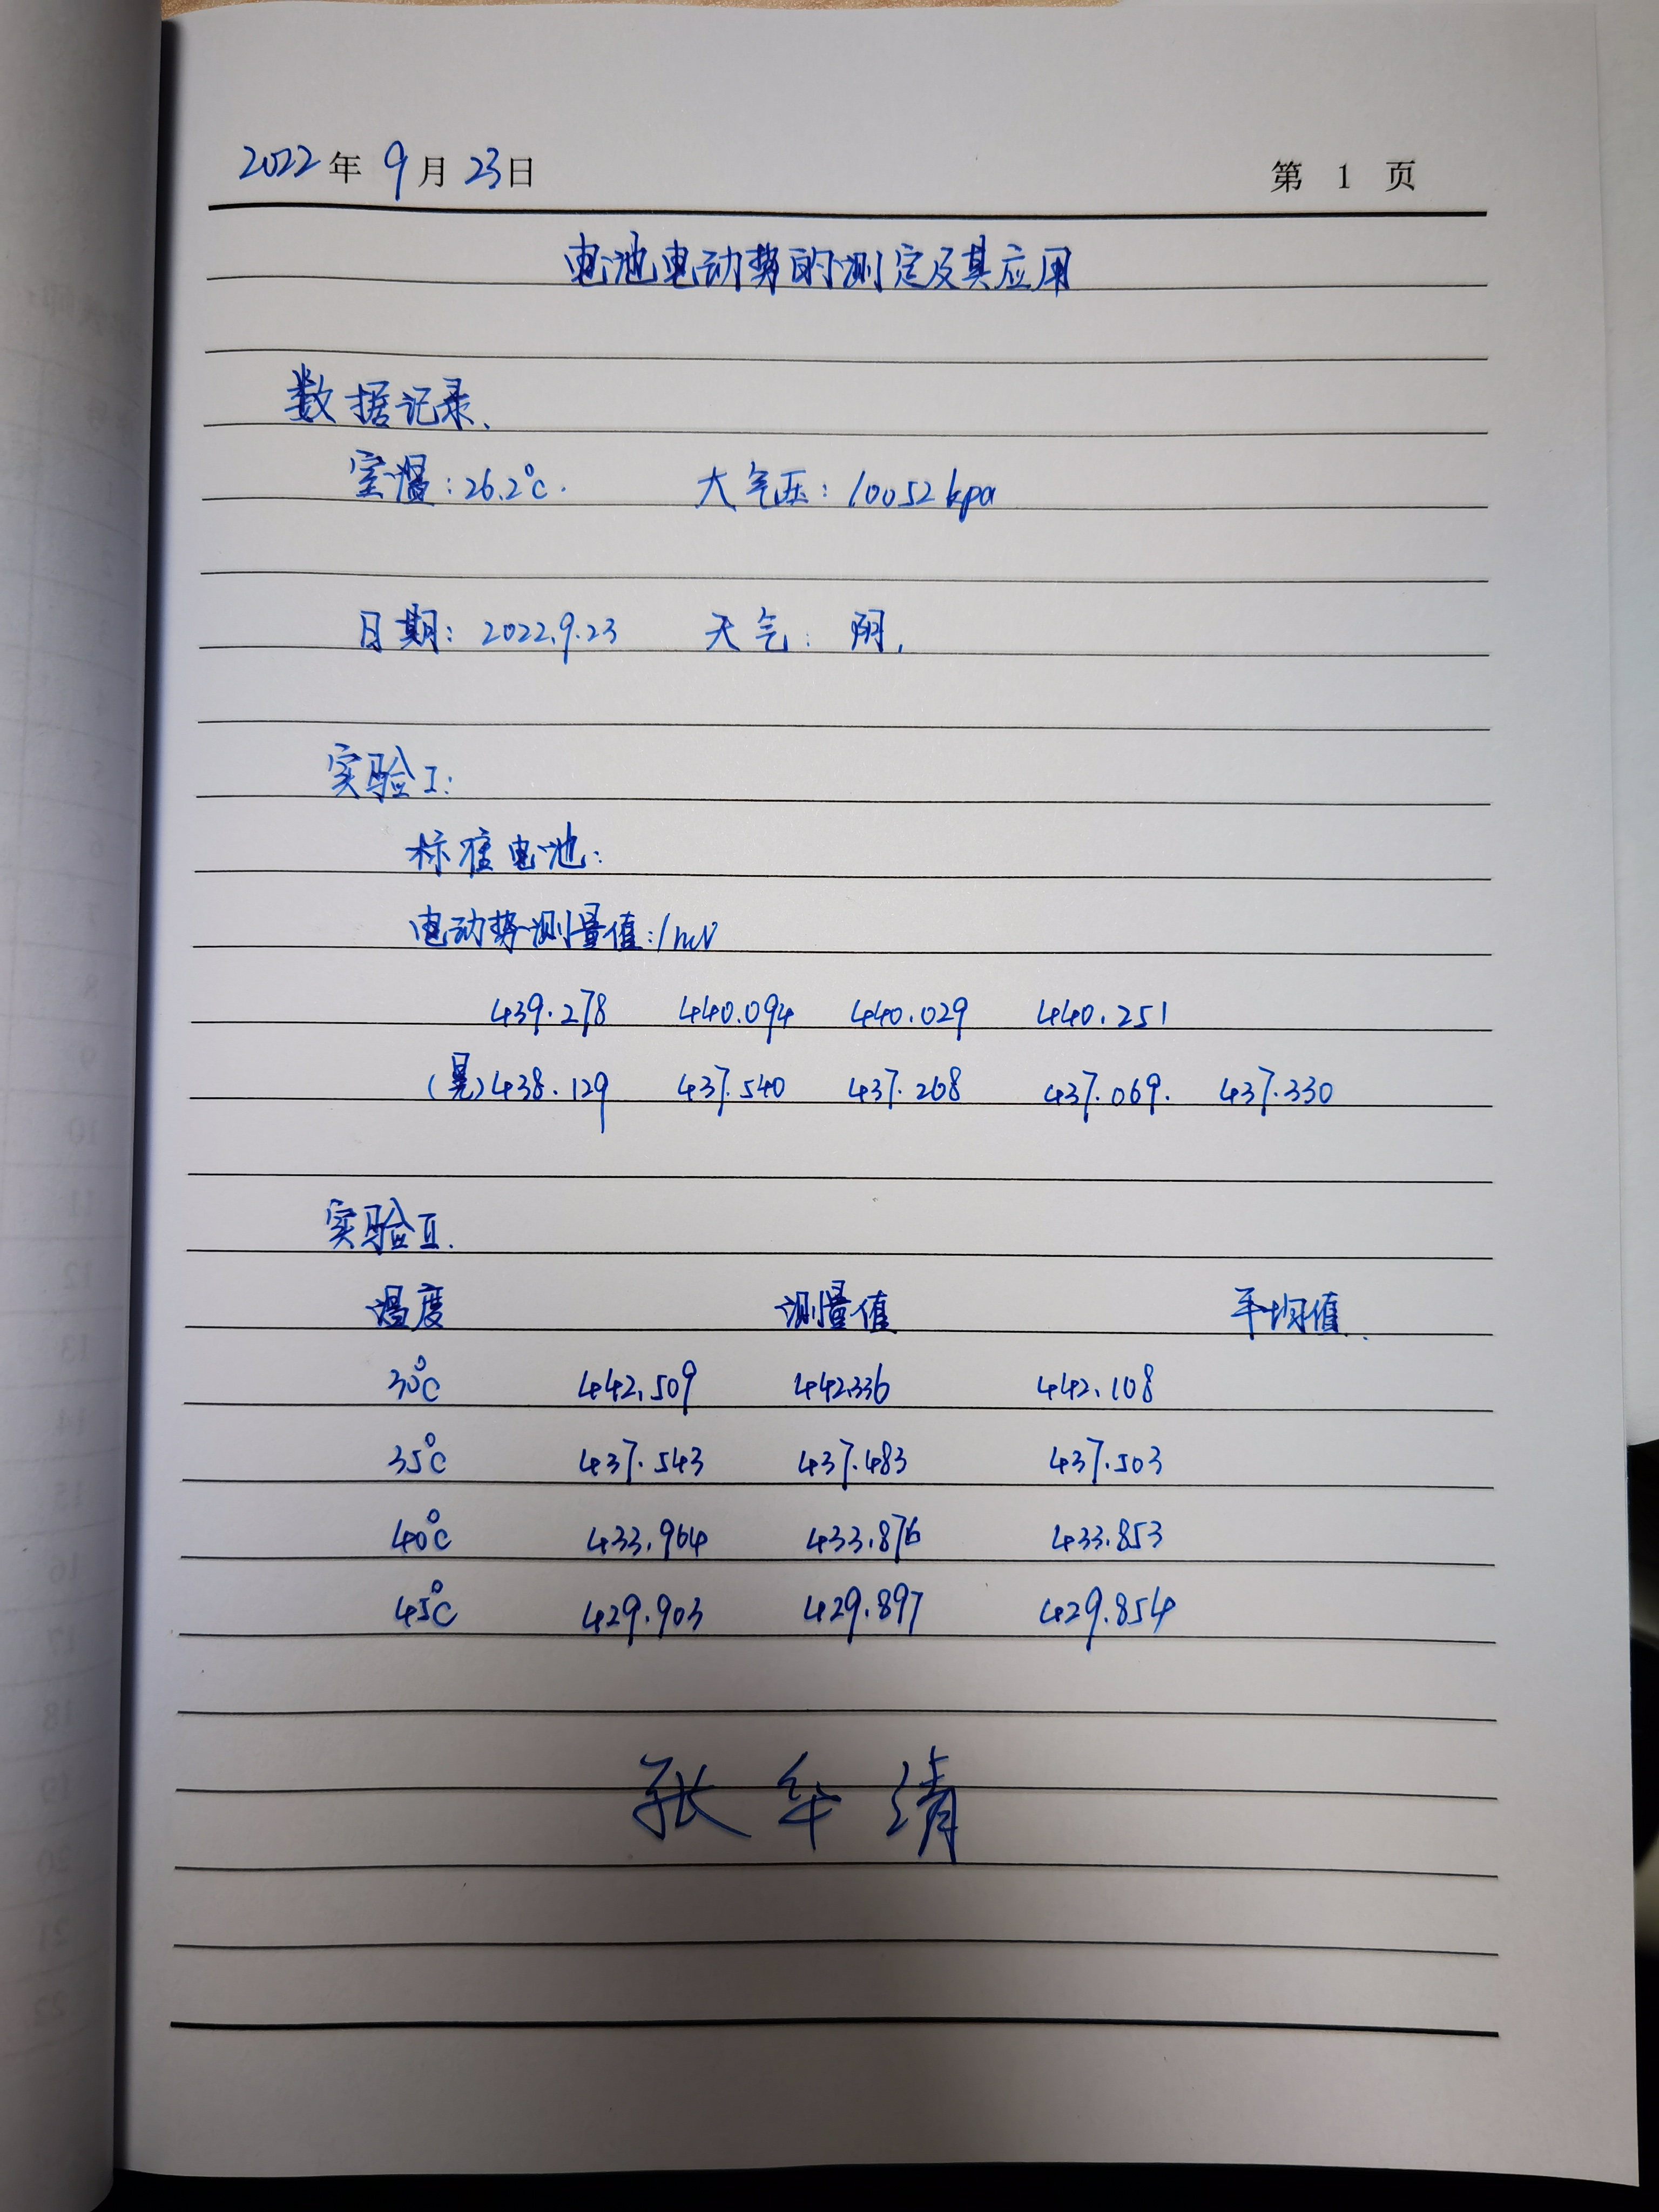
\includegraphics[width=1\textwidth]{实验6原始数据.jpg}
    \caption{实验6原始数据}
    \label{fig:2}
\end{figure}



\end{document}